%\documentclass[xetex,mathserif,serif]{beamer}
\documentclass{beamer}
\renewcommand{\tiny}{\fontsize{4}{14}\selectfont}

\usepackage{hyperref}
\usepackage{fontspec} 
\usepackage{xunicode} %Unicode extras!
\usepackage{xltxtra} %Fixes 
\usefonttheme{professionalfonts}
\setmainfont{Linux Libertine O}
%\setmonofont[Scale=0.86]{DejaVu Sans Mono}
\setmonofont{Liberation Mono}
%\setromanfont{Silkscreen}
%\setsansfont{DejaVu Sans}
\setsansfont{Droid Sans}

\usepackage[final,expansion=true,protrusion=true,spacing=true,kerning=true]{microtype}
\usetheme{openlab} 
\setbeamertemplate{navigation symbols}{}
\usepackage{graphicx}

\title[Students]{Open IT Lab} 
\author{Jarrell Waggoner} 
\institute[Open IT Lab] {Open IT Lab\\
  \medskip
      {\emph{waggonej@email.sc.edu}} }
\date{\today}

\newcommand{\putat}[3]{\begin{picture}(0,0)(0,0)\put(#1,#2){#3}\end{picture}}

\usebackgroundtemplate{
\includegraphics[width=\paperwidth]{../img/bg.png}}

% Videos/websites to show:
% About SFD: http://softwarefreedomday.org/
% Dictionary Definition: http://dictionary.reference.com/browse/open
% RSA Animate: http://youtu.be/u6XAPnuFjJc?t=6m44s
% Karen Sandler: http://youtu.be/nFZGpES-St8?t=2m26s
% My video
% Thing-O-Matic Video: http://www.flickr.com/photos/retrocactus/6044172663/
% Arduino projects: http://hacknmod.com/hack/top-40-arduino-projects-of-the-web/
% Free Content: http://questioncopyright.org/understanding_free_content
% Open Cola Ingredients: http://en.wikipedia.org/wiki/OpenCola_%28drink%29
% Creative Commons Selection: http://creativecommons.org/choose/

\begin{document}
\rm

{
  \usebackgroundtemplate{
\includegraphics[width=\paperwidth]{../img/bg-title.png}} 
  \begin{frame}
%    \titlepage
    \vspace{18em}

    \begin{center}\large{\textcolor{beamer@mygrey}{Jarrell Waggoner}}\end{center}

%    \begin{center}\small{\textcolor{beamer@mygreen}{waggonej@email.sc.edu}}\end{center}

%    \begin{center}\small{\textcolor{beamer@mygrey}{\today}}\end{center}
  \end{frame}
}

\begin{frame}
  \frametitle{About Me}
  \begin{LARGE}
    Jarrell Waggoner
  \end{LARGE}
  \begin{Large}
    \begin{itemize}
    \item Ph.D. candidate in computer science at the College of
      Engineering and Computing at USC
    \item Been writing software for 15 years
    \item Using open source and creating open content since 1998
    \item Created an open movie in 2006
    \item Teaching programming and software development using open source tools since 2007
    \item Website: \textcolor{beamer@myblue}{\href{http://www.malloc47.com}{http://www.malloc47.com}}
    \end{itemize}
  \end{Large}
\end{frame}

% \begin{frame}
%   \vspace{-1em}
%   \begin{center} 
\includegraphics[width=0.9\textwidth]{../img/sfd} \end{center}
%   \begin{large}
%     \begin{itemize}
%     \item Annual worldwide celebration of Free and Open Source
%       Software
%     \item 3rd Saturday of September \\ (occasionally overlaps with
%       International Talk Like A Pirate Day)
%     \item Over 500 individual celebrations around the world
%     \end{itemize}
%   \end{large}
% \end{frame}

\begin{frame}
  \begin{center}
    \begin{Huge}
      Software vs. Hardware
    \end{Huge}

    
\includegraphics[width=0.4\textwidth]{../img/tux-question-3}
    \end{center}
\end{frame}

\begin{frame}
  \begin{center} 
    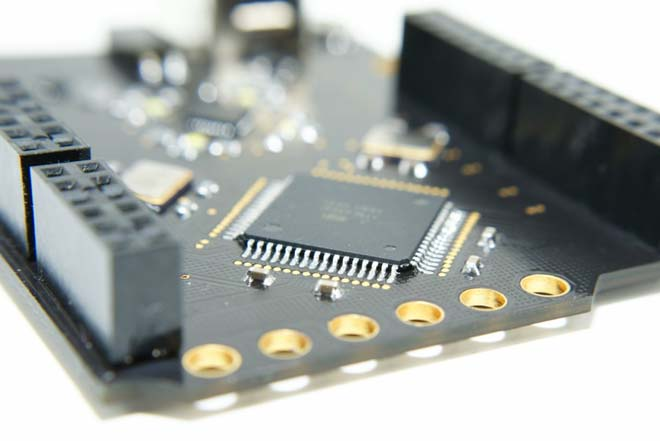
\includegraphics[width=0.7\textwidth]{../img/hardware}
    \begin{Huge} Hardware \end{Huge} 
  \end{center}
\end{frame}

\begin{frame}
  \frametitle{What is hardware?}
  \begin{center}
    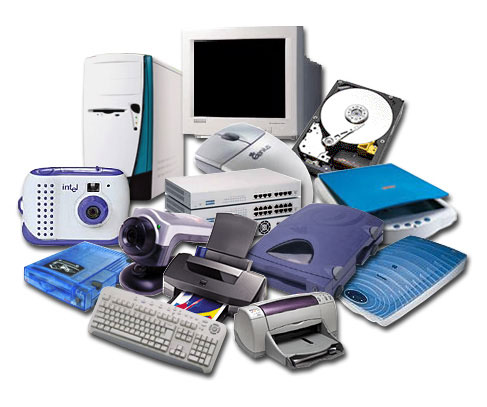
\includegraphics[width=0.4\textwidth]{../img/hardware-2}
  \end{center}
  \begin{itemize}
  \item The physical "stuff" that our electronics are made out of
  \item Costs lots of money in R\&D to create
  \item Requires tools and supplies to build that most people do not have
  \end{itemize}

\end{frame}

\begin{frame}
  \begin{center} 
    
\includegraphics[width=1\textwidth]{../img/software-words-3}
    \begin{Huge} Software \end{Huge} 
  \end{center}
\end{frame}

\begin{frame}
  \frametitle{What is software?}
  \begin{center}
    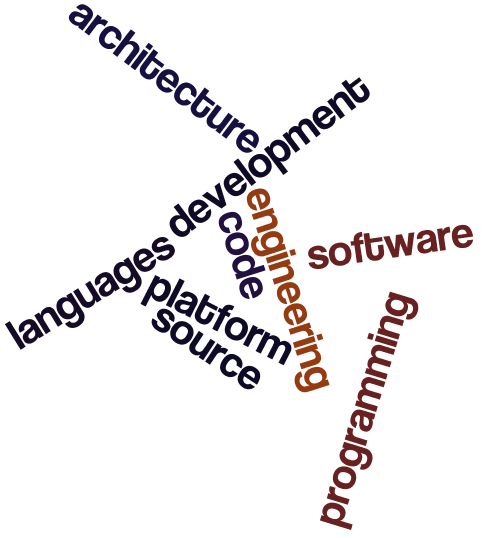
\includegraphics[height=0.6\textheight]{../img/software-words-4}
  \end{center}

    \only<1>{Think of Hardware as a \textcolor{beamer@myblue}{Television} and software as the \textcolor{beamer@myblue}{TV shows}. The TV show \textcolor{beamer@myblue}{director} and \textcolor{beamer@myblue}{actors} are all "programmers."}
    \only<2>{\textcolor{beamer@myblue}{Piano} as hardware and \textcolor{beamer@myblue}{sheet music} as software. The \textcolor{beamer@myblue}{composer} of the music is a "programmer."}

\end{frame}

\begin{frame}
  \frametitle{How is software made?}
  \begin{overlayarea}{\textwidth}{\textheight}
   \vspace{1em}

  \begin{center}
    \only<1>{Project $\rightarrow$ Programmer(s) $\rightarrow$ Code $\rightarrow$ Hardware}
    \only<2>{\textcolor{beamer@myblue}{Project} $\rightarrow$ Programmer(s) $\rightarrow$ Code $\rightarrow$ Hardware}
    \only<3>{Project $\rightarrow$ \textcolor{beamer@myblue}{Programmer(s)} $\rightarrow$ Code $\rightarrow$ Hardware}
    \only<4>{Project $\rightarrow$ \textcolor{beamer@myblue}{Programmer(s)} $\rightarrow$ Code $\rightarrow$ Hardware}
    \only<5>{Project $\rightarrow$ Programmer(s) $\rightarrow$ \textcolor{beamer@myblue}{Code} $\rightarrow$ Hardware}
    \only<6>{Project $\rightarrow$ Programmer(s) $\rightarrow$ Code $\rightarrow$ \textcolor{beamer@myblue}{Hardware}}
  \end{center}

  \only<1>{\vspace{4em} 

    A \textcolor{beamer@myblue}{programmer} writes \textcolor{beamer@myblue}{code} to solve a problem. This code can be \textcolor{beamer@myblue}{compiled} to run on specific \textcolor{beamer@myblue}{hardware}. Some software is only designed to be used by few people, and some software is designed to be given away to everyone, or sold for profit.}
  \only<2>{
    \begin{itemize}
    \item Identify a problem or business need
    \item Hire people to solve the problem
    \item Find management to lead the project
    \item Develop a plan to create the project
    \item Figure out how the team will work together
    \item Define the specifications of what has to be created
    \item Give tasks to the programmer(s) hired to work on the project
    \end{itemize}
  }
  \only<3>{
    \begin{itemize}
    \item Identify a problem or business need
    \item Hire people to solve the problem
    \item Find management to lead the project
    \item Develop a plan to create the project
    \item Figure out how the team will work together
    \item Define the specifications of what has to be created
    \item Give tasks to the programmer(s) hired to work on the project
    \end{itemize}
    \putat{85}{0}{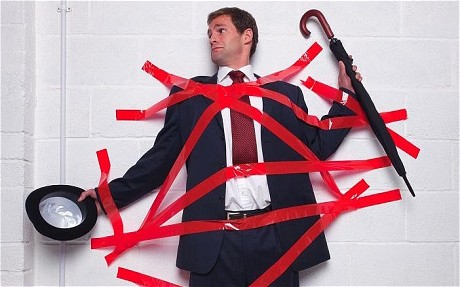
\includegraphics[width=0.5\textwidth]{../img/red-tape}}
    % \begin{center} 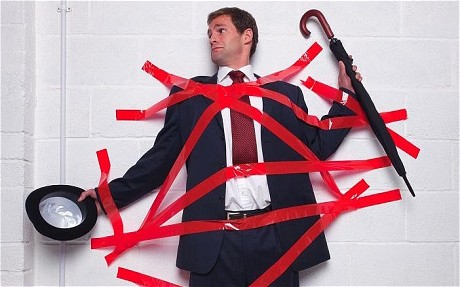
\includegraphics[width=0.75\textwidth]{../img/red-tape} \end{center}
  }
  \only<4>{
    \begin{center}
      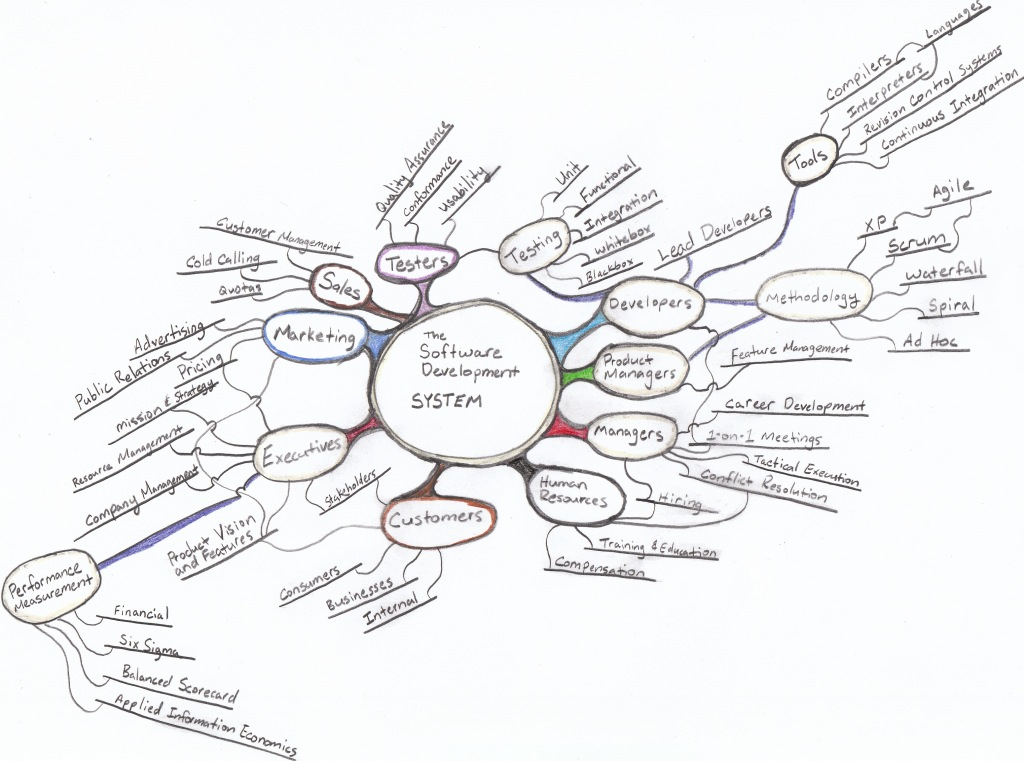
\includegraphics[width=0.75\textwidth]{../img/software-development}
    \end{center}
  }
  \only<5>{
    \begin{center}
      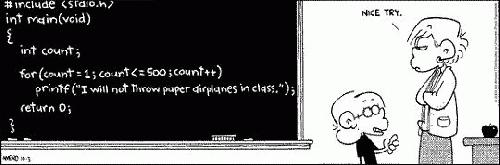
\includegraphics[width=0.65\textwidth]{../img/foxtrot}
      \begin{itemize}
      \item Instructions for the hardware to carry out
      \item Many \textcolor{beamer@myblue}{languages} to choose from
        that different computers understand
      \item 
      \end{itemize}
    \end{center}
  }
  \end{overlayarea}
\end{frame}

\begin{frame}
  \frametitle{Introduction}
  \begin{center}\begin{LARGE}What does it mean to be Open?\end{LARGE}\end{center}
\end{frame}

\begin{frame}
  \frametitle{What does the dictionary say?}
  \begin{center}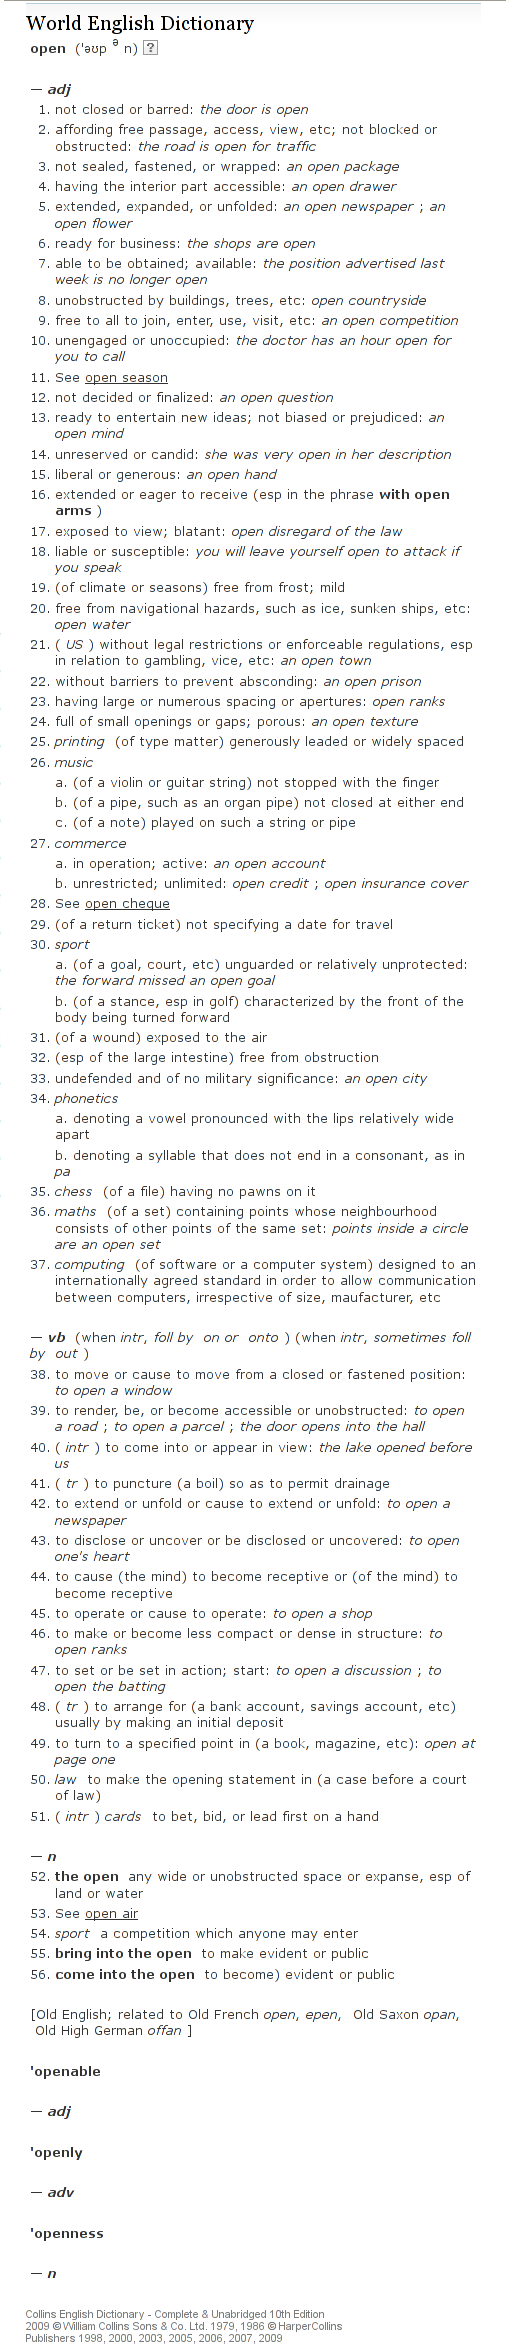
\includegraphics[height=0.8\textheight]{../img/dictionary}\end{center}
\end{frame}

\begin{frame}
  \frametitle{What does the dictionary say?}
  \begin{center}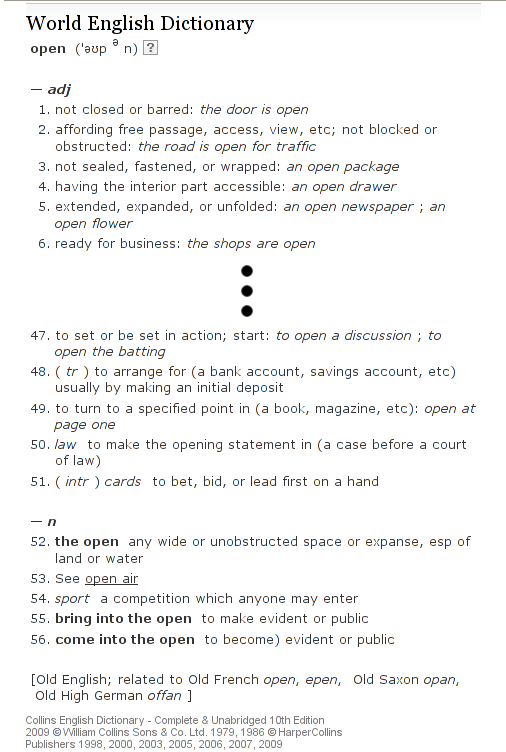
\includegraphics[height=0.8\textheight]{../img/dictionary2}

    \href{http://dictionary.reference.com/browse/open}{http://dictionary.reference.com/browse/open}
  \end{center}
\end{frame}

\begin{frame}
  \frametitle{Our Definition}
  \begin{overlayarea}{\textwidth}{\textheight}
    \begin{center}
      
\includegraphics[width=0.35\textwidth]{../img/freedom}

      \begin{LARGE}
        The freedom to share, explore, reproduce, and contribute ideas
        and projects based on these ideas
      \end{LARGE}
    \end{center}
    \vspace{1em} \only<2>{\begin{block}{So...}  If a project is open,
        you can \textcolor{beamer@myblue}{explore and learn} from it,
        \textcolor{beamer@myblue}{share} it with others,
        \textcolor{beamer@myblue}{duplicate} it and
        \textcolor{beamer@myblue}{remix} your own variants, and work
        with the creators to make it
        \textcolor{beamer@myblue}{better}!
      \end{block}}
  \end{overlayarea}
\end{frame}

\begin{frame}
  \frametitle{Who, What, Where, When...}
  \begin{overlayarea}{\textwidth}{\textheight}
    \vspace{1.5em}
    \begin{description}
    \item[Who uses and contributes?]
      \only<2->{Everyone, young and old!}
    \item[Where from?] \only<3->{Anywhere in the world, thanks to the internet}
    \item[What do they contribute?] \only<4->{Software, hardware, and content}
    \item[When did this start?] \only<5->{1983? 1991? Earlier? Later?}
    \end{description}
    \begin{center}
      \only<1>{
\includegraphics[width=0.4\textwidth]{../img/tux-question-3}}
      \only<2>{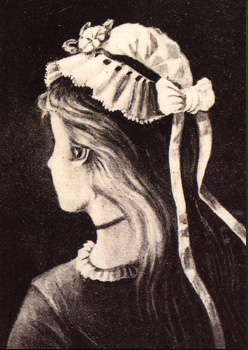
\includegraphics[width=0.25\textwidth]{../img/optical-illusion-2}}
      \only<3>{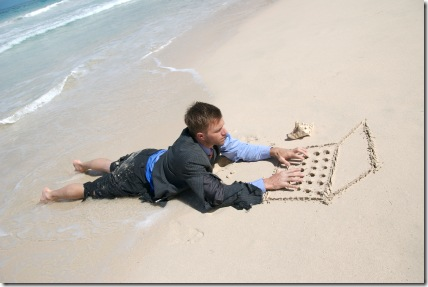
\includegraphics[width=0.5\textwidth]{../img/anywhere}}
      \only<4>{
        \vspace{2em}
        
\includegraphics[height=0.15\textheight]{../img/opensource}
        \hspace{2em}
        
\includegraphics[height=0.15\textheight]{../img/opensourcehardware.png}
        \hspace{2em}
        
\includegraphics[height=0.15\textheight]{../img/cc.png}}
      \only<5>{
\includegraphics[width=0.4\textwidth]{../img/tux-clock}}
    \end{center}
  \end{overlayarea}
\end{frame}

\begin{frame}
  \frametitle{Open vs. Free vs. Free AND Open}

  Take software, for an example: 

  \begin{description}
  \item[Free Software] Freedom to do what you like with the software (e.g. give it away, create your own version, etc.)
  \item[Open Source] Ability to see how the software was created, and to share and improve it
  \item[Free Open Source Software / FOSS] A way to say both things at the same time!
  \item[Free Libre Open Source Software / FLOSS] Adds the ``libre'', which makes sure we know what kind of ``free'' we're talking about: free as in ``freedom'' not free as in no cost
  \end{description}
\end{frame}

\begin{frame}
  \frametitle{Free}
  \begin{LARGE}
    "Free software is a matter of liberty, not price. To understand
    the concept, you should think of free as in free speech, not as in
    free beer."

    \vspace{1em}

    \textemdash Richard Stallman
  \end{LARGE}

\end{frame}

\begin{frame}
  \frametitle{Free (no cost) may not be good...}
  \begin{LARGE}
    "If you are not paying for it, you’re not the customer; you’re the product being sold."

    \vspace{1em}

    \textemdash MetaFilter poster
  \end{LARGE}
\end{frame}

\begin{frame}
  \frametitle{What can be open?}
  \begin{columns}
    \column{0.45\textwidth}
    \begin{center}
      \begin{LARGE}Software\end{LARGE}
      
      \vspace{5em}

      \begin{LARGE}Hardware\end{LARGE}

      \vspace{5em}

      \begin{LARGE}Content\end{LARGE}
    \end{center}
    \column{0.45\textwidth}
    \begin{center}
      
\includegraphics[width=0.4\textwidth]{../img/opensource}

      \vspace{1em}

      
\includegraphics[width=0.4\textwidth]{../img/opensourcehardware.png}

      \vspace{1em}

      
\includegraphics[width=0.8\textwidth]{../img/cc.png}
    \end{center}
  \end{columns}

\end{frame}

\begin{frame}
  % Cut?
  \frametitle{Formal Definition}
  \begin{center}
    \begin{block}{Software}
      Allows free distribution, modification the source code, allows
      derived works, does not discriminate or have limiting license
      restrictions\textemdash\textcolor{beamer@myblue}{\href{http://opensource.org/docs/osd}{opensource.org}}
    \end{block}

    \begin{block}{Hardware}
      hardware whose design is made publicly available so that anyone
      can study, modify, distribute, make, and sell the design or
      hardware based on that design\textemdash\textcolor{beamer@myblue}{\href{http://freedomdefined.org/OSHW}{OSHW}}
    \end{block}

    \begin{block}{Content}
      A piece of content or data is open if anyone is free to use,
      reuse, and redistribute it--subject only, at most, to the
      requirement to attribute and
      share-alike\textemdash\textcolor{beamer@myblue}{\href{http://www.opendefinition.org/}{opendefinition.org}}

      \vspace{1em}
      
      Open content encourages the 4Rs: Reuse, Revise, Remix,
      Redistribute\textemdash\textcolor{beamer@myblue}{\href{http://www.opencontent.org/definition/}{opencontent.org/definition}}
    \end{block}
  \end{center}
\end{frame}

\begin{frame}
  \frametitle{When?}

  \begin{description}
  \item[Predates computers:] Some things have always been free (recipes, camp-fire songs, etc.)
  \item[1983:] GNU Project launched by Richard Stallman
  \item[1991:] Linux is released by Linus Torvalds
  \item[Late 90s:] The dot-com era--open source becomes big!
  \item[1998:] Open Source Initiative founded
  \item[1998:] Netscape launched as open source (later became Firefox)
  \item[1999:] Source Forge, the leading open project repository, is launched
  \item[2004:] Ubuntu launched by Mark Shuttleworth
  \item[2007:] Dell announces that it will offer Ubuntu preinstalled on its laptops
  \item[2007:] Open Handset Alliance announces the Android Operating System, based on Linux, for use on phones
  \item[2009:] Microsoft submits device drivers to the Linux Kernel under an open source license
  \end{description}
\end{frame}

\begin{frame}
  \frametitle{... and Why?}
  \begin{columns}
    \column{0.45\textwidth}
    
\includegraphics[width=0.9\textwidth]{../img/bunny-2}
  %   \begin{Large}Businesses \end{Large}
  %   \begin{itemize}
  %   \item Less management, as the open projects are self-managed
  %   \item Free to customize to fit business needs
  %   \item Open projects adhere to open standards, so you can use your data with any open project that supports the standard
  %   \item More secure, as open projects can be vetted by many more experts
  %   \end{itemize}
    \column{0.45\textwidth}
    \begin{Large}Individuals\end{Large}
    \begin{itemize}
    \item Learn and collaborate with smart people with similar interests
%    \item It's okay if it's not finished or half done
    \item They're paid to work on open projects by their company
    \item They're expected to spend part of their time on personal projects, and they want to share their work (e.g. Google)
    \item It's like giving your time to charity--it's for a good cause, and your work can live on long after you're gone
    \end{itemize}
  \end{columns}
%TODO: picture
%http://www.youtube.com/watch?v=u6XAPnuFjJc
%http://www.catb.org/esr/writings/cathedral-bazaar/
\end{frame}

% \begin{frame}
%   \frametitle{Video}
%   \begin{center}
%     \begin{LARGE}
%       \href{http://youtu.be/u6XAPnuFjJc?t=6m44s}{http://youtu.be/u6XAPnuFjJc?t=6m44s}
%     \end{LARGE}
%   \end{center}

% \end{frame}

% http://youtu.be/u6XAPnuFjJc?t=6m44s

\begin{frame}
  % http://www.youtube.com/watch?v=nFZGpES-St8
  \frametitle{Open vs. Proprietary}
  \begin{center}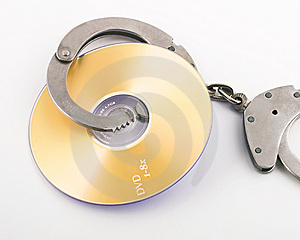
\includegraphics[width=0.4\textwidth]{../img/proprietary}\end{center}  \begin{Large} Proprietary \end{Large}
  \begin{itemize}
  \item May cost \textcolor{beamer@mygreen}{money} (not necessarily though!)
  \item \textcolor{beamer@mygreen}{Not} allowed to see how it works
  \item You're only \textcolor{beamer@mygreen}{licensed} to use it and don't own it
  \item Sometimes less \textcolor{beamer@mygreen}{secure}, as fewer experts get to look at how it was created

  \end{itemize}

\end{frame}

\begin{frame}
  \frametitle{Open vs. Proprietary}
  \begin{Large} Proprietary \end{Large}
  \begin{itemize}
  \item May \textcolor{beamer@mygreen}{lock} users into a product that won't work with other systems once they've learned it
    
  \item Can add arbitrary \textcolor{beamer@mygreen}{restrictions} (like taking away features or keeping you from using it under arbitrary circumstances) to protect their product or get you to upgrade (e.g. Kindle, PS3, etc.)
  \end{itemize}

  \begin{center}
\includegraphics[width=0.25\textwidth]{../img/tuxmoney}\end{center}
  \begin{block}{Remember}
    You can still sell open source software! Red Hat sells a distribution of Linux--but you can get the source code and get the exact same code for free.
  \end{block}
\end{frame}

\begin{frame}
  \frametitle{About sums it up...}
  \begin{center}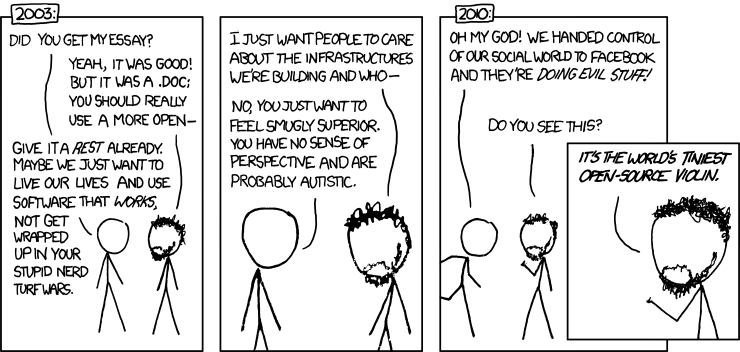
\includegraphics[width=1\textwidth]{../img/violin}\end{center}
  \begin{footnotesize}
    \textcolor{beamer@myblue}{\href{http://xkcd.com/743/}{http://xkcd.com/743/}}
  \end{footnotesize}
\end{frame}

\begin{frame}
  \begin{center} 
    
\includegraphics[width=1\textwidth]{../img/software-words-3}
    \begin{Huge} Software \end{Huge} 
  \end{center}
\end{frame}

\begin{frame}
  \frametitle{Software Examples}
  Examples of open projects:

  \begin{itemize}
  \item Software
    \begin{description}
    \item[Linux] Operating system that can be modified to work on just
      about any device
    \item[Firefox] Web browser that runs on any operating system (both
      open source operating systems and proprietary operating systems)
    \item[Open Office] Complete office suite that produces documents
      that can be opened by any system
    \item[Blender] 3D computer graphics software to model and render CGI images and video
    \end{description}
    \end{itemize}
\end{frame}

\begin{frame}
  \frametitle{Linux}
  \begin{columns}
    \column{0.45\textwidth}
    \begin{LARGE}
      Linux
    \end{LARGE}
    \begin{itemize}
    \item Released in 1991 by Linux Torvalds
    \item Created as a free alternative to Unix
    \item Now runs on
      \begin{itemize}
      \item MACs \& PCs
      \item Video game consoles
      \item PDAs and Phones (Android)
      \item GPSs and Cars
      \item Servers / Supercomputers
      \end{itemize}
    \end{itemize}
    \column{0.45\textwidth}
      \begin{center}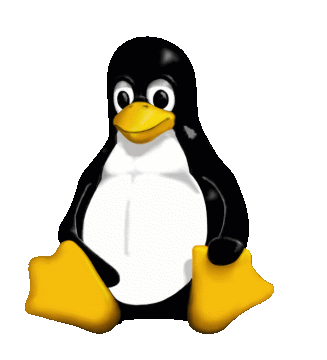
\includegraphics[width=0.5\textwidth]{../img/tux}\end{center}
      
      \begin{center}
\includegraphics[width=0.5\textwidth]{../img/ubuntu}\end{center}
  \end{columns}
\end{frame}

\begin{frame}
  \frametitle{Who Contributes to Linux?}
  All of these companies actively work to make Linux better (and since Linux is Open Source, we all get to benefit from their work):
  \begin{columns}
    \column{0.45\textwidth}
    
    \begin{Large}
      \begin{itemize}
      \item Red Hat
      \item Novell
      \item IBM
      \item Intel
      \item Oracle
      \item Google
      \item $\ldots$
        even 
\includegraphics[width=0.3\textwidth]{../img/microsoft}!
      \end{itemize}
    \end{Large}

    \column{0.45\textwidth}
    \begin{center}
      
\includegraphics[width=0.3\textwidth]{../img/redhat}

      
\includegraphics[width=0.4\textwidth]{../img/novell}

      
\includegraphics[width=0.3\textwidth]{../img/ibm}

      
\includegraphics[width=0.3\textwidth]{../img/intel}

      
\includegraphics[width=0.4\textwidth]{../img/oracle}

      
\includegraphics[width=0.4\textwidth]{../img/google}
    \end{center}
  \end{columns}
  \begin{center}
    You've used Linux if you've ever Googled anything!
  \end{center}

\end{frame}

\begin{frame}
  \frametitle{Blender}
  \begin{center} 
\includegraphics[width=0.8\textwidth]{../img/blenderex} \end{center}
  \begin{itemize}
  \item Fully featured 3D modeler, renderer, and compositer
  \item Works on all major operating systems, and even on old hardware
    \\ (I was using blender back in 2001!)
  \item Is free, compared to commercial software that cost 1000s of
    dollars, so anyone can start learning how to use it right away
  \item Has state-of-the-art features comparable to similar
    proprietary tools--you can do studio-quality work in Blender!
  \end{itemize}
\end{frame}

\begin{frame}
  \frametitle{Blender Example}
    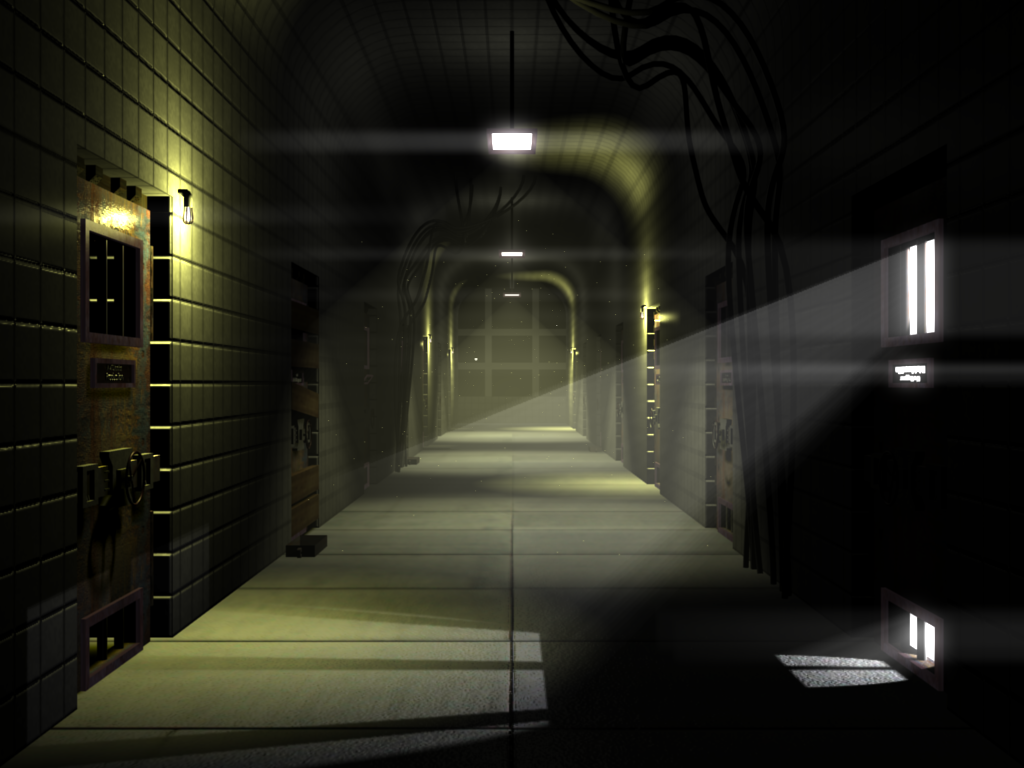
\includegraphics[width=\textwidth]{../img/blendermine}
\end{frame}

\begin{frame}
  \begin{center} 
    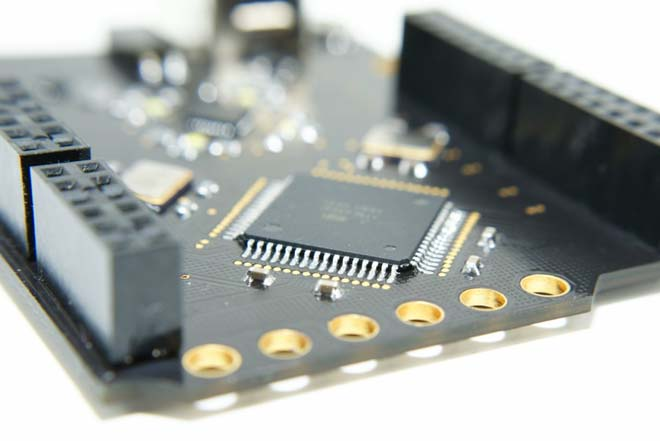
\includegraphics[width=0.7\textwidth]{../img/hardware}
    \begin{Huge} Hardware \end{Huge} 
  \end{center}
\end{frame}


\begin{frame}
  \frametitle{Hardware Examples}
  Examples of open projects:

  \begin{itemize}
  \item Hardware
    \begin{description}
    \item[Thing-O-Matic] A \textcolor{beamer@myblue}{3D} Printer that
      can produce 3D objects out of a special plastic
      \textcolor{beamer@myblue}{reproduce} itself by printing the
      necessary components to build a new device.
    \item[Arduino] Electronic prototyping platform for creating
      interactive electronic objects.
    \end{description}
  \end{itemize}
\end{frame}

\begin{frame}
  \frametitle{Makerbot Thing-O-Matic}
  \begin{center} 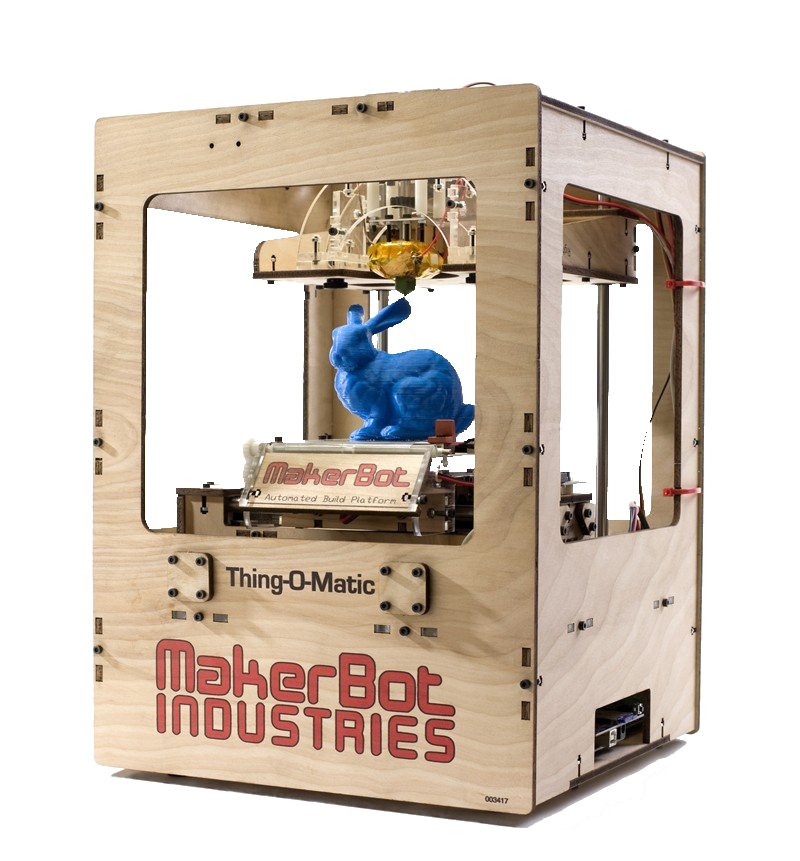
\includegraphics[width=0.4\textwidth]{../img/thing-o-matic} \end{center}
  \begin{itemize}
  \item A \textcolor{beamer@myblue}{3D} Printer that can produce 3D
    objects out of a special plastic
  \item Can be built by anyone if they have the parts
  \item Can \textcolor{beamer@myblue}{reproduce} itself by printing the
    necessary components to build a new device.
  \end{itemize}
\end{frame}

\begin{frame}
  \frametitle{Makerbot Thing-O-Matic}
  \begin{center} 
    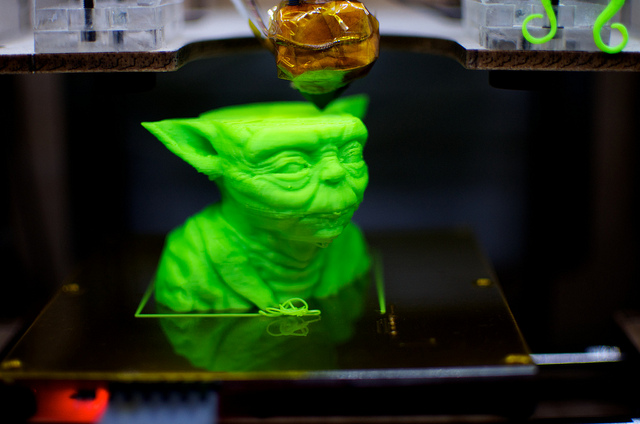
\includegraphics[width=0.5\textwidth]{../img/yoda}

    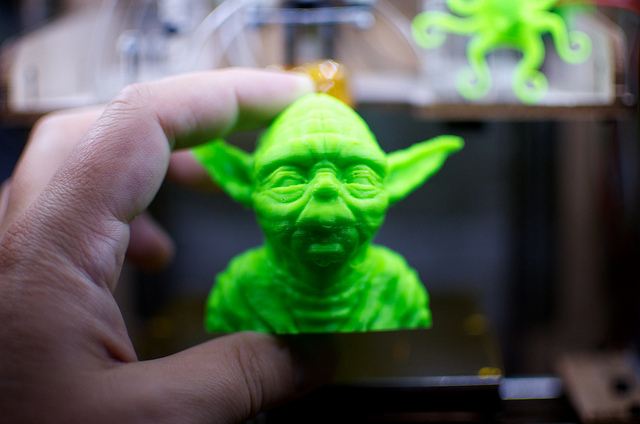
\includegraphics[width=0.5\textwidth]{../img/yoda-2} 
  \end{center}
\end{frame}

% http://www.flickr.com/photos/retrocactus/6044172663/

\begin{frame}
  \frametitle{Arduino}
  \begin{center} 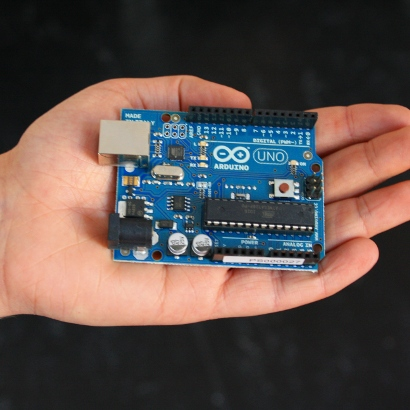
\includegraphics[width=0.4\textwidth]{../img/arduino} \end{center}
  \begin{itemize}
  \item Small, programmable \textcolor{beamer@myblue}{microcontroller}
  \item Open hardware, so all the build specs are available to build
    it yourself (you can also buy pre-built Arduinos)
  \item Been used in lots of different projects, and is small enough to be embedded in RC cars, musical instruments, and even clothing
  \end{itemize}
\end{frame}

% http://hacknmod.com/hack/top-40-arduino-projects-of-the-web/

\begin{frame}
  \begin{center} 
    
\includegraphics[height=0.7\textheight]{../img/content-king}

    \begin{Huge} Content \end{Huge} 
  \end{center}
\end{frame}

% http://questioncopyright.org/understanding_free_content
\begin{frame}
  \frametitle{Content Examples}
  Examples of open projects:
  \begin{itemize}
  \item Content
    \begin{description}
    \item[Wikipedia] An online encyclopedia that can be freely accessed (and modified!) by anyone
    \item[Project Gutenberg] An archive of public domain content that is made available in long-lasting open formats that
    \item[data.gov] Open Government initiative to release government information as open content
    \item[OpenCola] A softdrink that can be made by anyone (the recipe
      is freely available)
    \end{description}
  \end{itemize}
\end{frame}

\begin{frame}
  \frametitle{Wikipedia}
  \begin{center} 
\includegraphics[height=0.35\textheight]{../img/wikipedia}\hspace{1em} 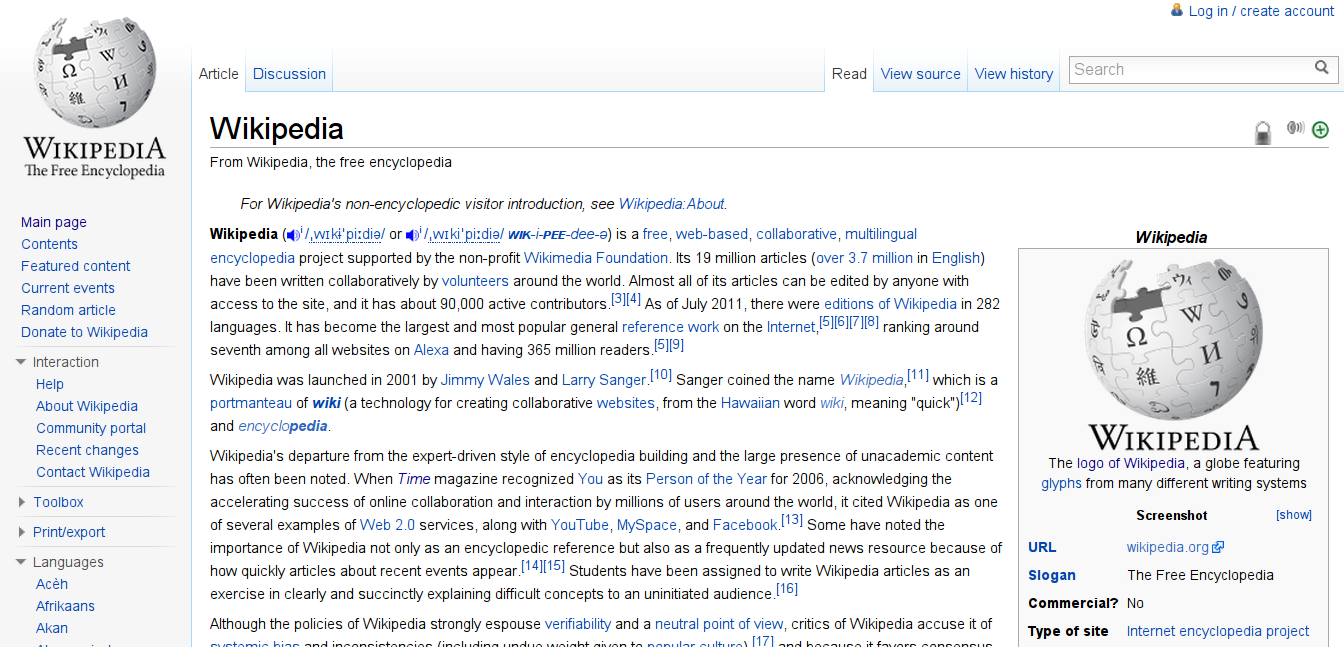
\includegraphics[height=0.35\textheight]{../img/wikiwiki} \end{center}
  
  \begin{itemize}
  \item Online encyclopedia that anyone can edit
  \item 19 million articles in 282 languages
  \item 90,000 active contributors (vs. 72 for Britannica)
  \item First to move away from ``expert-written'' encyclopedias and let anyone contribute to their open content
  \item More timely than any encyclopedia (online or offline)
  \item Would take over 7 years to read the current Wikipedia!
  \end{itemize}
\end{frame}

\begin{frame}
  \frametitle{data.gov}
  \begin{center} 
\includegraphics[height=0.1\textheight]{../img/data-gov} \hspace{2em} \includegraphics[height=0.2\textheight]{../img/data-gov-site} \end{center}
  
  \begin{itemize}
  \item Home of the US Government's Open Data initiative
  \item Work with
    \begin{itemize}
    \item state/local governments to make their content open
    \item open software developers to make it easier to get access to government data
    \item individuals to help them get be informed and involved in government
    \end{itemize}
  \item Helped launch
    \begin{itemize}
    \item 29 Open State Government initiatives
    \item 11 Open U.S. City Government initiatives
    \item 172 Open Government Agencies
    \item 21 International Open Government initiatives
    \end{itemize}

  \end{itemize}
\end{frame}

\begin{frame}
  \frametitle{OpenCola}
  \begin{center} 
    \includegraphics[height=0.3\textheight]{../img/opencola} \hspace{2em} \includegraphics[height=0.3\textheight]{../img/opencola-ingredients} 
  \end{center}
  \begin{itemize}
  \item Soft drink whose recipe is freely available
  \item Anyone can modify the recipe as they please
  \item No "secret" ingredients, so you know its safe
  \item Originally designed to help explain the idea of free software
  \end{itemize}
\end{frame}

% http://en.wikipedia.org/wiki/OpenCola_%28drink%29

\begin{frame}
  \frametitle{So Why Open Source?}
  \begin{description}
  \item[Everyone] Cost, freedom, compatibility
  \item[Students] Accessible information, Projects to build on, Resources to learn from
  \item[Teachers] Opportunity to close the digital divide, 21st skills easier than ever to teach
  \item[Entrepreneurs] Stability, security
  \end{description}
\end{frame}

% \begin{frame}
%   \frametitle{Advocates of Open Source}
%   \begin{description}
%   % \item[Electronic Frontier Foundation] Helps to protect the rights of
%   %   open projects to help make sure they stay open for everyone
%   \item[Free Software Foundation] 
%   \end{description}
% \end{frame}

\begin{frame}
  \frametitle{How to Get Involved}
  \begin{itemize}
  \item Software
    \only<2>{
    \begin{enumerate}
    \item Write software
    \item Release it with an Open Source license
      \begin{itemize}
      \item GNU Public License (GPL): Is now, and will forever be free
      \item BSD License: Is free, but can be used in commercial projects too
      \end{itemize}
    \end{enumerate}}
  \item Hardware
    \only<3>{
    \begin{enumerate}
    \item Build hardware
    \item Make the schematics available to everyone with an open source license
    \end{enumerate}}
  \item Content
    \only<4>{
    \begin{enumerate}
    \item Write, direct, conduct, compose, assemble, cook, generate$\ldots$
    \item Make your work available with a \textcolor{beamer@mygreen}{Creative Commons} License of your choice
      \begin{itemize}
      \item Attribution
      \item Attribution-ShareAlike
      \item Attribution-NoDerivs
      \item Attribution-NonCommercial
      \item Attribution-NonCommercial-ShareAlike
      \item Attribution-NonCommercial-NoDerivs 
      \end{itemize}
    \item Find stuff related to your project to make available
% http://creativecommons.org/choose/
    \end{enumerate}}
  \end{itemize}


  \begin{center}
      \only<2>{\includegraphics[height=0.2\textheight]{../img/gpl}}
      \only<4>{\includegraphics[height=0.2\textheight]{../img/creative-commons}}
      \only<5>{
        \begin{Large}
        You can simply add an open license (GPL, Creative Commons, etc.) to something to make it open, just like you can add a \copyright to restrict it and make it "closed."
        \end{Large}}

  \end{center}

\end{frame}

\begin{frame}
  \begin{center}
    \includegraphics[height=0.5\textheight]{../img/linux-lab}    

    \vspace{1em}

    \begin{Huge}
      Lab Tour!
    \end{Huge}
  \end{center}
\end{frame}

\begin{frame}
  \frametitle{Explore}
  \begin{block}{Goal}
    Explore open source!
  \end{block}

  Challenges:
  \begin{itemize}
  \item[$\square$] Start \textcolor{beamer@mygreen}{LibreOffice Impress} and create a slide
    describing yourself
  \item[$\square$] Find all the planets (and Pluto!) in
    \textcolor{beamer@mygreen}{Celestia}
  \item[$\square$] What's the fasted speed you can get up to in
    \textcolor{beamer@mygreen}{Extreme Tux Racer}?
  \item[$\square$] Create a few spheres in \textcolor{beamer@mygreen}{Blender}
  \item[$\square$] Draw a picture in
    \textcolor{beamer@mygreen}{Inkscape},
    \textcolor{beamer@mygreen}{GIMP}, or
    \textcolor{beamer@mygreen}{TuxPaint} (make sure to save it!)
  \item[$\square$] Use \textcolor{beamer@mygreen}{FreeMind} to list all the open software and content you've tried or seen
  \item[$\square$] In \textcolor{beamer@mygreen}{Scratch}, try to program the cat to move in a continuous loop

  \end{itemize}

\end{frame}

\end{document}
